\documentclass[10pt,twocolumn,letterpaper]{article}

\usepackage{cvpr}
\usepackage{times}
\usepackage{epsfig}
\usepackage{graphicx}
\usepackage{amsmath}
\usepackage{amssymb}
\graphicspath{ {images/} }
% Include other packages here, before hyperref.

% If you comment hyperref and then uncomment it, you should delete
% egpaper.aux before re-running latex.  (Or just hit 'q' on the first latex
% run, let it finish, and you should be clear).
\usepackage[breaklinks=true,bookmarks=false]{hyperref}

\cvprfinalcopy % *** Uncomment this line for the final submission

\def\cvprPaperID{****} % *** Enter the CVPR Paper ID here
\def\httilde{\mbox{\tt\raisebox{-.5ex}{\symbol{126}}}}

% Pages are numbered in submission mode, and unnumbered in camera-ready
%\ifcvprfinal\pagestyle{empty}\fi
\setcounter{page}{1}
\begin{document}

%%%%%%%%% TITLE
\title{Visual Speech Reconstruction from Lip Motions}

\author{Mouse Lee\\
{\tt\small jl27@princeton.edu}
\and
Jonathan Metzman\\
{\tt\small jmetzman@princeton.edu}
\and
Bo Moon\\
{\tt\small bhmoon@princeton.edu}
}

\maketitle
%\thispagestyle{empty}

%%%%%%%%% ABSTRACT
\begin{abstract}
  The aim of this project is to develop a program for visual speech recognition by identifying spoken words based on lip motions. These lip motions are tracked using an external library for Constrained Local Models. The lip motion of a user is extracted using this library, then compared against a precompiled database consisting of lip motions corresponding to certain words. We present algorithms for speech detection and calculating an error metric between two different lip motions, as well as discussing various obstacles and assumptions present in handling visual data, such as unwanted geometric transformations of the face. The performance of this program is tested using a limited dictionary and several users.
\end{abstract}

%%%%%%%%% BODY TEXT
%------------------------------------------------------------------------
\section{Motivation}
\subsection{Why do this}
We found VSR to be a worthy problem for a couple of reasons. A VSR system can be used to recognize speech in scenarios where only visual data is kept, such as in Closed Circuit TV recordings. A more common use case than recognizing speech in video recording without audio is recognizing speech in a recording with a large amount of background noise. Background noise makes audio based speech recognition considerably more difficult, so a vision or hybrid speech recognition system could be more accurate in noisy scenarios \cite{Dupont}.

\subsection{What makes this difficult}
We constructed a system that can determine which words, from a predefined set of words, or dictionary, are being said.

A VSR system must be able to determine the words that are being spoken based on the motion of a user's mouth. This can actually be quite hard in the real world because of things like differences between the lighting or camera in the testing and training data. Recognizing the speech of real people can be difficult because of factors such as moving the face, different lip shapes, and even different pronunciations of the same word among various people.

There also commonplace computer vision obstacles that make tracking the motion of the mouth more difficult such as makeup, glasses, facial hair, and even the teeth and tongue.

We believe that our system is resilient to some of these challenges, and performs well in real conditions. One important feature we attempt for practical reasons is for our system to be capable of recognizing the speech of a user without requiring training on data supplied by the same user. Other issues such as poor lighting and occlusion are commonplace problems for most visual systems, including our program; we think a speech recognition system that also used audio data would be most robust in these scenarios.



%------------------------------------------------------------------------
\section{Related Work}
\subsection{What has been done}
Speech recognition has gone from academic research interest to an essential part of the way user interact with computing devices ~\cite{Lison:2014:SDS:2677339.2659891}.
Most of these technologies rely solely on acoustic data. However, an obvious drawback of these systems is that their performace is severly degraded by noise ~\cite{Cooke2001267}. Research has shown that systems that use visual data in place of, or in addittion to audio data, can significantly outperform systems that only use audio data in the presence of noise ~\cite{Lison:2014:SDS:2677339.2659891}.

\subsection{What are the problems}
Most other research, with a few exceptions focuses mainly on acoustic recognition, with visual recognition used as a secondary means of recognition. We thought that using a purely vision based approach would be an interesting challenge, and provide some of the advantages outlined above.
Another difference between our approach and those of most other VSR systems is that most of them try to detect visual phenomes, or visemes, rather than actual words.
While this approach is more generalizable and would allow detection of words that the system has not been explicitly trained on, we suspected that this approach may be less accurate for recognizing specific words than the approach we decided to take.
One study that used this method was able to acheive 72.73\% recognition of vowels, since the percentage would drop for specific words we felt the usefulness of this approach is quite limited for many use cases ~\cite{Viseme}.
A final advantage our implementation has over nearly any other implementation is portability. Since our implementation can run in web browsers it can run on virtually every platform in common use today.


%-------------------------------------------------------------------------
\section{Algorithm}

\subsection{Overview}
First we will present an outline of how the program operates, and then afterwards discuss major problems, assumptions, and algorithms. The program is outlined as follows:
\begin{enumerate}
\item Initialize dictionary: The user first must compile a database of known words and the associated lip motions so queries may be made later.
\item Begin video capture, initialize mouth threshold and nose bridge length: The program displays a live feed and also initializes two parameters. The program also uses an external library to track the user’s lips.
\item Detect when word has been spoken: The program detects when the user has spoken a word.
\item Capture all relevant frames: After the user has finished speaking, all frames associated with the word are stored to be used as a query against the database.
\item Compare query to each word in the database: A metric is computed to determine how similar the query is to a word in the database as measured by their lip motions.
\item Use modified k nearest neighbors to return the best matching word: The computed metrics are used to find a group of the most similar words, which is then used to find the best matching word.
\end{enumerate}

\subsection{Obtaining and Representing Data}
Our program makes use of the Javascript clmtracker library (https://github.com/auduno/clmtrackr).
It uses Constrained Local Models, a technique for finding statistical estimates of coordinates on an object based on its shape, combined with trained support vector machines to identify and track many facial landmarks, as seen below.

\begin{figure}[h]
\centering
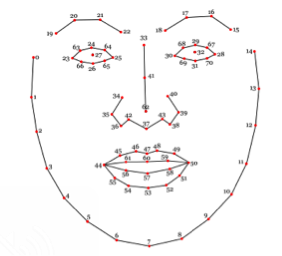
\includegraphics{bo1}
\caption{The various facial landmarks detected by the CLM tracker.}
\end{figure}

The CLM tracker library is used to identify and track 18 points on the lip. These 18 points are represented by and pixel coordinates for each frame; thus, the program represents each frame as an array of 18 points, also interpreted as a matrix of 18 rows and 2 columns:
\begin{equation}
  f = [(x_1, y_1), (x_2, y_2), \ldots, (x_{18}, y_{18})]
\end{equation}
The program represents a word as an array of all consecutive frames in which the user was speaking, plus 25 additional frames before and after speaking as a buffer to capture initial and final lip motions. For instance, if the program detected that the user spoke for frames, then the word is stored as
\begin{equation}
  w = [f_1, f_2, \ldots, f_{n+49}, f_{n+50}]
\end{equation}

where the first 25 frames are immediately before when the program detects the start of speech, and the last 25 frames are immediately after when the program detects the end of speech. The value 25 was chosen since that is the average frame rate of the webcam used.
\subsection{Geometric Transformations}
The points obtained by the CLM tracker are stored in pixel coordinates. As such, these coordinates are highly sensitive to various geometric transformations such as rotations and translations, which make the points difficult to handle for algorithms and computations. Ideally, lip point coordinates will change only when there is lip motion, as in speech. We can implement some measures to reduce or ignore undesirable motion.
\subsubsection{Translations}
Translations occur when the user moves his/her face around the screen (assuming the face does not turn/rotate).

\begin{figure}[h]
\centering
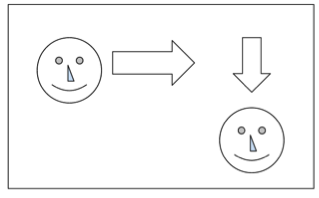
\includegraphics{bo2}
\caption{An example of translation.}
\end{figure}

Consider the pixel coordinates of the right corner of the lip in the figure above. Even though the lip is in the same position on the face, the pixel coordinates before and after the translation are different because the entire face has moved. However, note that the position of that particular point has not changed relative to any other point on the face since all points on the face have been translated the same amount. As such, we can make lip point coordinates resistant to translations by transforming the coordinates into a new coordinate system with the origin somewhere on the face. This way, translating the face would translate the entire coordinate system, so no lip point coordinates would be changed.
In our program we accomplish this by imposing a coordinate system on the tip of the nose, although any facial feature would have worked. Specifically, for every lip point $(x, y)$ in pixel coordinates and the pixel coordinates of the tip of the nose $(nose_x, nose_y)$, the new coordinates are a position vector in the form
\begin{equation}
  p = (nose_x - x, nose_y - y)
\end{equation}

\subsubsection{Scaling}

\begin{figure}[h]
\centering
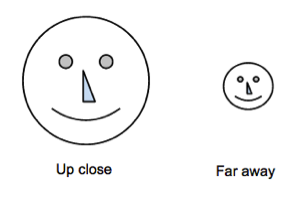
\includegraphics{bo3}
\caption{An example of scaling.}
\end{figure}

The face in the video changes scale when the user changes his/her distance to the camera, e.g. the face becomes larger when the user is closer and shrinks when the user is farther away. The coordinates of  are still sensitive to scaling. However, when the face changes scale, all lengths on the face are scaled by the same amount, so the face before and after scaling are geometrically similar. Therefore, by using simple geometry, we can find ratio of lengths on the face to calculate this scaling factor.
The CLM tracker also tracks the nose bridge. During the calibration phase, the nose bridge length of the user face is recorded. Later, during the testing phase, the scaling factor is calculated by
\begin{equation}
  s = \frac{\textrm{recorded nose length}}{\textrm{current nose length}}
\end{equation}

where the the recorded and current nose lengths are the nose lengths obtained during calibration and in the current frame, respectively. Afterwards, this scaling factor is used to scale all lip points per frame as such:
\begin{equation}
  p' = s \times p = (s(nose_x - x), s(nose_y - y))
\end{equation}
\subsubsection{Rotations}
Rotations occur when the user rotates his/her face. This is a significant problem since if the user’s face rotates too much, the coordinate system based on the nose would not rotate with the face, so coordinates of each point would be incorrect. The simplest solution to this problem is to avoid having rotations altogether. As such, we require that the user’s face looks straight on into the camera, i.e. the optical axis of the camera is orthogonal to the plane of the face, and the head is not tilted.
Calculating $p'$ is a way to make the coordinates less sensitive to changes so that we do not have to be concerned with geometric problems in later algorithms.
However, in practice $p'$ still changes slightly due to these transformations. For instance, when the user translates his/her face in the video, the user will naturally turn to face the camera the entire time. This rotation has been observed to cause the coordinates of $p'$ to fluctuate by 4-6 units, which is not very significant.
Nevertheless, the program performs best when the user’s face is in the center of the screen, looking straight at the camera without rotating, and as stationary as possible.
\subsection{Calibration}
Calibration is the procedure of compiling a dictionary of known words so that queries can be made later to find the best matching word. There are several problems of calibration that will be discussed later, such as how speech is detected and what particular words ought to be stored in the dictionary.

Calibration is performed before making any queries, but after calibration is done it does not need to be repeated. The program works best if the same user who calibrates the dictionary also makes the queries, so it is recommended that a new user to calibrate his/her own dictionary. During calibration, the user will prepare a list of words he/she wishes to be in the dictionary. The user then speaks each of these words multiple times to camera. The program detects the speech and records an array of frames and prompts the user to type what word was spoken. Afterwards, this array and string are stored as a pair in a database. In the end, if there are $W$ words and each is said $T$ times, the database will have $WT$ entries where each entry is a tuple of an array of frames and a string, but there will only be $W$ unique strings in the database. These duplicate strings exist for use in a modified k nearest neighbors algorithm, to be discussed later.
As for implementation details, the database used in our program was \hyperref[https://www.firebase.com/]{''Firebase''} and we had 5 distinct words that were each repeated 6 times for a total of 30 entries in the dictionary.
\subsection{Video Capture and Speech Detection}
There are some basic miscellaneous assumptions associated with the capture and display of video: The user and camera should be in a well-lit but not too bright setting; the face should be visible (glasses and hair are acceptable but nothing covering the mouth); the user should not speak too quickly, and slowly enough so that the video shows the lip moving without skipping or blurring motions.

The program needs to determine when the user has started and finished talking so that all frames containing lip motions can be stored. First, to determine whether the mouth is open or closed, we use the distance between the centers of the top and bottom lips, which we refer to as the mouth height. Before speech detection begins, we require the user to have his/her mouth closed and record the square of the mouth height. During speech detection, for each frame we calculate the square of the current mouth height. If it is greater than the recorded value, then this means the mouth is open; otherwise, the mouth is closed. We use squared distances because this makes the program more sensitive to small changes in motion; for instance, if the camera observes the lips move by 2 pixels, then the program registers this motion as 4 units.

For speech detection, we use a combination of counting frames and threshold values. In short, speech is detected if this sequence of events is followed:
\begin{enumerate}
\item Mouth opens: Determined when the previous frame detects a closed mouth and current frame is open.
\item Mouth remains open for at least a certain (small) number of frames: If the mouth is not open for at least that many frames, most likely the program accidentally detected a false open mouth. Otherwise the mouth is still in motion right now.
\item Mouth remains closed for a certain (relatively large) number of frames: If the mouth is not closed for at least that many frames, most likely the mouth only momentarily closed to pronounce a plosive sound (e.g. “baboon”), so this does not count as the user being done speaking. Otherwise this indicates the mouth is done speaking.
\end{enumerate}
An array is used to store the relevant frames in the meantime, and when the user has finished speaking, these frames are processed.

\subsection{Comparing Words}
When the query is obtained, it is stored as an array of frames $q$. Furthermore, all words in the dictionary database are stored as a tuple of a string representing the word itself and an array of frames spoken during calibration. In order to find the best matching word in the dictionary, we need some way to measure the similarity between the query array $q$ and a dictionary word array $w$.

We can describe this problem geometrically, but to simplify the description, we will consider only one point on the lip, then later generalize to all 18 lip points. For now, let $q = (q_1, q_2, q_3, \ldots, q_n)$ be a sequence of coordinates such that $q_i = (x_i^q, y_i^q)$ are the coordinates of a lip point during the ith frame of speaking a query, and there are $n$ such coordinates in total. Similarly, let $w = (w_1, w_2, w_3, \ldots, w_m)$ be a sequence of frames such that $w_i = (x_i^w, y_i^w)$ are the coordinates of a lip point during the ith frame of speaking a dictionary word, and there are $m$ such coordinates in total.

\begin{figure}[h]
\centering
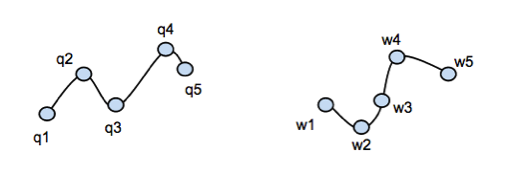
\includegraphics{bo4}
\caption{Two possible curves if the coordinates in $q$ and $w$ are connected.}
\end{figure}

If the coordinates stored in the array $q$ are plotted and connected, they form the curve that the lip point travels across those frames; the same is true for $w$. As such, the problem of finding the similarity between a query and a word can be posed as determining how “similar” two curves are. If $n = m$ (that is, if the query and word are the exact same number of frames) then a natural metric to use is the sum of squared distances between the corresponding coordinates:
\begin{equation}
  error(q,w)=\sum_{i=1}^{n} \| q_i-w_i \| ^2
\end{equation}
where $||q_i-w_i|| = \sqrt{(x_i^q - x_i^w)^2 + (y_i^q - y_i^w)^2}$ is the distance function. With this, a smaller error corresponds to a more similar curve. However, this metric is problematic because it is exceedingly rare that a user will say two words for exactly the same number of frames, even if those words were the same. The inconsistency in the length of the arrays also makes it difficult to apply a machine learning algorithm, since a feature vector would have to be engineered to compensate for arrays of variable dimensions. As such, another metric is needed.

\begin{figure}[h]
\centering
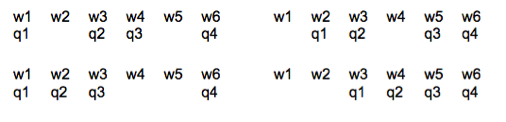
\includegraphics{bo5}
\caption{Four possible arrangements of $q$ and $w$ with $n=4$ and $m=6$.}
\end{figure}

Consider the two curves $q$ and $w$ for $n < m$ (that is, the query is spoken for fewer frames than the word in the dictionary). Since $q$ is shorter than w, it is possible to align $q$ in various ways such that the relative ordering of the elements of $q$ is preserved but the corresponding elements in $w$ are different, as in the figure. For each of these alignments, we can still calculate the sum of squared distances by taking pairs of corresponding entries, despite the fact that $q$ is shorter than $w$.  As such, we define a similarity metric between $q$ and $w$ to be the minimum possible score obtainable among all possible alignments of $q$ to $w$ and taking the sum of squared distances. Interpreted geometrically, this metric is calculated by splitting the curve $q$ into multiple strands, then trying to align each of those strands against $w$ while maintaining the correct order of strands, as in Figure 6. Furthermore, we must attempt all possible splits and all possible number of strands that can be made from $q$.

\begin{figure}[h]
\centering
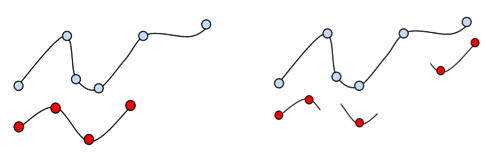
\includegraphics{bo6}
\caption{Blue curve is $w$, red curve is $q$. On the right, $q$ has been split to find a relatively good alignment to $w$, and ordering of the split curves is preserved.}
\end{figure}

To calculate this metric, we use a dynamic programming algorithm. Let $M(i,j)$ be the similarity metric between the sequences $(q_1, q_2, q_3, \ldots, q_i)$ and $(w_1, w_2, w_3, \ldots, w_j)$. In other words, $M(i,j)$ is the smallest score obtainable by aligning the first $i$ coordinates of $q$ to the first $j$ coordinates of $w$.  We will try to align $q$ to $w$ starting from the end, then align recursively. For $q_i$, there are only two possible options when aligning it to $w_j$: either $q_i$ is aligned with $w_j$, or it is not aligned. If $q_i$ is aligned with $w_j$, these two coordinates form a pair that contributes an amount of $\|q_i - w_i\|$ to the final score furthermore, the problem is now reduced to aligning $(q_1, q_2, q_3, \ldots, q_i)$ to $(w_1, w_2, w_3, \ldots, w_j)$. If $q_i$ is not aligned with $w_j$, then this means that $q_i$ must be aligned with some coordinate of $w$ that comes before $w_j$; this is described by the subproblem $(q_1, q_2, q_3, \ldots, q_i)$ and $(w_1, w_2, w_3, \ldots, w_j)$ Thus, we can represent these relationships as
\begin{equation}
  M(i,j)=\textrm{min}\{M(i-1,j-1)+\| q_i-w_j \| ^2, M(i,j-1) \}
\end{equation}
The base cases are occur when $i > j$ or $i = j = 0$. When $i > j$, this means that there are too many coordinates in $q$ to align against w, so it is impossible to make an alignment; thus, $M(i, j) = \infty$. When $i = j = 0$, this is the trivial case of aligning an empty sequence against an empty sequence, so $M(i, j) = M(0, 0) = 0$. The time and space complexity of this algorithm is $O(nm)$ since this dynamic programming algorithm uses memoization to fill an $n$ by $m$ table (note this table would be a lower triangular matrix because of the base cases).

Using this similarity metric, we can compute the score between $q$ and $w$ to be $M(i, j)$ for when $n < m$ (we will discuss the case when $n \ge m$ shortly). This is only for the simplified case of one lip point, but we can generalize this to all 18 lip points. Let $q = (f_1^q, f_2^q, f_3^q, \ldots f_n^q)$ be a sequence of frames that constitutes the spoken query, where $f_i^q = [(x_1^q, y_1^q), (x_2^q, y_2^q), \ldots, (x_{18}^q, y_{18}^q)]$ is the array of 18 lip points as defined earlier. Define $w$ analogously. The similarity metric is now
\begin{equation}
  M(i,j)=\textrm{min}\{M(i-1,j-1)+\| f_i^q-f_j^w \|, M(i,j-1) \}
\end{equation}
where we define
\begin{equation}
\| f_i^q-f_j^w \| = \sum_{1}^{18}(x_i^q-x_i^w)^2+(y_i^q-y_j^w)^2
\end{equation}
or in words, the sum of squared distances between all 18 pairs of corresponding lip points in two frames.

Since $M(i, j)$ is the minimum sum of squared differences between curves, it is actually a geometric error metric between $q$ and $w$.  This error metric can be computed for the query compared against each word in the dictionary. As such, a word with a relatively small error metric means that it has a similar shaped path to the query.

It appears this algorithm works only for $n < m$, or when the query is spoken faster than the word being compared. One obvious solution would be to swap $q$ and $w$ and call $M(m, n)$ instead. However, this does not address the main weakness of this algorithm: if $n << m$, it is likely that $M(m, n)$ will be very low, so $q$ will be calculated to be very similar to $w$.  This is because there are many possible alignments if the query is spoken much faster than the word, so it is more likely for a smaller score to be found. As such, the real issue is making sure that the ratio of $n$ to $m$ is an appropriate amount.

To use this algorithm, we want $am<n<bm$ for some $0<a<b<1$; in other words, we want the ratio of $n$ to $m$ to be within a certain small range. If it is the case that $n>bm$, then we can sample the query by removing frames until $n<bm$. This is analogous to taking a video clip of a person speaking and accelerating the playback by a small factor. We must remove $k=n-bm$ frames, so we remove every $\lfloor n/k  \rfloor$th frame. A value of $b=.8$ was chosen empirically for our program.

If $n<am$, then we must add $l=am-b$ frames, so we pad the query by duplicating every $\lfloor n/l \rfloor$th frame. This would be analogous to taking a video clip and decelerating it by a small factor. (With the particular set of words used in this program, this latter measure did not make a significant difference, so it was not used.) Note that this technique of accelerating/decelerating the frames works under the assumption that when people speak faster or slower the speed difference is uniform; for instance, when someone says the word “orthogonal” quickly, it would not be pronounced with the first three syllables said quickly and the last syllable drawn out.

One advantage of this algorithm is that it can handle instances where the query and dictionary word are not spoken for the same number of frames, which happens for virtually all queries since it extremely unlikely for a user to speak a word for the exact same amount of time as another word. A disadvantage is that when a very short query is padded to match a long word, or if a long query is sampled to match a short word, it may be possible that these processes were not the best transformations to use to compare different length words.

\subsection{Finding the best match}

Although it is possible to find the word with the least error when compared to the query, there is a problem of what dictionary word arrays are to be stored in the database. For instance, one might think that during the calibration phase the user could speak the same word multiple times, take the average coordinates of each point for each frame, then store that array of frames, but it is not feasible to find an “average” motion because as mentioned before it is extremely rare for a person to pronounce two words for the exact same number of frames.

As such, we use a modified form of the k nearest neighbors algorithm, where for our program $k=5$. The dictionary’s database actually stores multiple copies of each word. For instance, there can be five arrays of frames, each one labeled as the word “orthogonal” because the user said that word five times during calibration. Consequently, we can compute the error metric for every word, including duplicates, in the dictionary, then among the top 5 the word with the highest frequency is determined. For instance, if the top five scoring words were hummingbird, koala, hyena, koala, and crocodile, the best match would be koala. This is not quite the same as k nearest neighbors since none of these points have features or attributes for a proper machine learning to be used, and the metric that is computed between two words is relevant only to that particular pair.

For our implementation, we used the following words in our dictionary: hyena, koala, platypus, hummingbird, crocodile. Each word was spoken 6 times so the dictionary contained 30 instances total. It is difficult to choose a set of words that is representative of the English language, so for such a preliminary, tentative evaluation, we selected a group of words that would help the performance of our algorithm. Specifically, these words are not too short—all are multisyllabic—and the lip motions for each word visually appear distinct from each other.


\section{Analysis}

When the same user who calibrates the dictionary also makes the queries, the output is very accurate. However, when there is any kind of cross use between different users—whether it is a user making queries to a dictionary he/she did not calibrate, or a dictionary that is calibrated by multiple people at the same time—the results are unsurprisingly poor. Reasonably, this is most likely because a person has his/her own idiosyncratic lip motion when speaking, in addition to different lip shapes and sizes. As such, results would predictably be best when the same user who calibrates the dictionary also makes the query, so this program is extremely user specific. Furthermore, some words that were misidentified were wrong but understandably so. For instance, the suffix of hummingbird, “mingbird”, has a very similar lip motion to the entire word “platypus”. For “crocodile” which was identified many times, this phenomenon probably occurred due to a mix of having different lip shapes, enunciations, and perhaps the lip motion for “crocodile” is on average similar to the rest of the words.

However, there were several problems with the evaluation. Only a small dictionary of few copies per word was used. Furthermore, we purposely selected that particular set of words to help the performance of the algorithm. These problems are due to some limitations of the nature of the problem. For one, it is difficult to select a group of words that is representative of the various lip motions of the English language. In addition, many instances of each word in the dictionary ought to be acquired to improve its performance, although this would require a very long, intensive calibration procedure. In addition, it is important to consider what to consider correct or incorrect by the program. For instance, the words “heft” and “cleft” have the same lip motions but are different words; even a human reading somebody’s lips could not distinguish them. As such, the program should not be penalized for such words, but identifying such pairs of words would require gathering much data.

There are some ways to improve the algorithm performance. The dynamic programming algorithm used may not have been an effective metric. One possibility would be to use a hidden Markov model or other statistical or machine learning tool to find the best matching word based off of coordinates. In addition, having a procedure to “normalize” words or arrays of frames may reduce error; for instance, finding geometric transformations to make coordinates resistant to translations, scaling, and rotations. A method for making queries and words the same number of frames would also help. Furthermore, it may be possible to engineer an appropriate feature vector from the lip motions so that proper machine learning techniques can be applied.

For the evaluation procedure, a more extensive dictionary comprised of a larger vocabulary of more instances each would make results more reliable. Furthermore, it would be interesting to see results of cross use with more users instead of just three people. Also, the algorithm would probably not perform well for shorter words since there would be less lip motion involved, but it would still be of interest to see the error rate in this case and understand how it could be reduced.

A possible next step for this algorithm would be to match syllables instead. It would be a similar mechanic to the current program: certain subsets of frames would correspond to a spoken syllable, and the program would have to find the most likely syllable spoken from the given lip motions. An issue with this is that syllables are also marked by tongue motion, so it would not be completely visible from video. However, if some procedure could at least approximate when syllables are spoken, then perhaps one approach would be to use a Bayesian network to find the most likely sequence of syllables that was spoken given the observed event of lip motions, then string the syllables together to produce a word.

{\small
\bibliographystyle{ieee}
\bibliography{LipReadingBib}
}

\end{document}
